%! Author = R2D2 Team 3
%! Date = 14/04/2020

% Preamble
\documentclass[11pt]{article}
\usepackage{hyperref}
\usepackage[official]{eurosym}

\usepackage{graphicx}
\usepackage{tabularx}
\graphicspath{ {./Images/} }

\usepackage{array}

\usepackage{natbib}

\usepackage{xcolor}

\usepackage{color}
\usepackage{colortbl}

\bibliographystyle{apalike}
\renewcommand{\refname}{\section{Referenties}}

\renewcommand{\contentsname}{Inhoudsopgave}

\newenvironment{definition}
    {
        \renewcommand{\arraystretch}{1.2}
        \begin{tabular}{>{\bfseries}l >{\em}p{0.7\textwidth}}
    }
    {
        \end{tabular}
        \renewcommand{\arraystretch}{1}
    }

\newcolumntype{Y}{>{\centering\arraybackslash}X}

\newcommand{\todo}[1]{\textcolor{red}{\emph{#1}}}


\title{Gebruik van Photoplethysmography om hartslag en zuurstofsaturatie te meten in rampgebieden}

\author{\emph{R2D2 Team 3} \and Finn Fonteijn \and Youri de Vor}

% Document
\begin{document}

    \begin{titlepage}
        \centering
        \maketitle
        
\includegraphics[height=0.6\textheight]{Images/vision.jpg}
        \clearpage
    \end{titlepage}


    \clearpage
    \tableofcontents

    \clearpage

    \section{Abstract}\label{sec:abstract}
    \todo{TODO, hier de abstract}

    \section{Voorwoord}\label{sec:voorwoord}
    Dit onderzoek wordt uitgevoerd in opdracht van de Hogeschool Utrecht, voor het project R2D2 2020.
    Bij dit project wordt er een ICT-bedrijf gesimuleerd.
    De werkgroep waaronder dit onderzoek valt is Team 3:\\
    \\

    \emph{
    \begin{tabularx}{\textwidth}{YYY}
        Niels Post & Otto de Visser & Amrit Malhi\\
        Menno van der Jagt & Youri de Vor & Finn Fonteijn\\
        Vincent van Setten & Oscar Kromhout
    \end{tabularx}
    \vspace{1em}
    }

    \section{Inleiding}\label{sec:inleiding}
    Het gebruik van een pulse oximeter geeft je belangrijke informatie over een aantal vitale functies van een slachtoffer. 
    Afhankelijk van de gekozen manier om deze meting uit te voeren, kan dit op een snelle, goedkope en niet-invasieve manier.
    In dit onderzoek kijken we naar verschillende meetmethoden en of deze geschikt zijn voor onze applicatie, letters B en C van de ABCDE methode voor eerste hulp. 
    Letters B en C staan voor breathing en circulation. 
    Vervolgens zullen wij kijken naar de verschillende sensoren die op de markt beschikbaar zijn, en de meest geschikte kiezen voor ons project.


    \section{Probleemstelling}\label{sec:probleemstelling}
    \todo{TODO, ik heb hier de probleemstelling van het voorstel gezet. Is dat goed zo?}
    In een rampgebied bevinden zich hulpbehoevende slachtoffers.
    Er is niet genoeg medisch personeel om iedereen te behandelen.
    Sommige slachtoffers bevinden zich op slecht begaanbare locaties.
    Het medisch team beschikt niet over de juiste middelen om een beeld te krijgen bij het aantal, de locatie en de toestand van de slachtoffers.
    Om snel de toestand van een slachtoffer te controleren is onder andere het meten van de zuurstofverzadiging en hartslag een vereiste.
    Het medisch personeel beschikt niet over voldoende data om systematisch de meest hulpbehoevende slachtoffers hulp te bieden.

    \section{Begrippenlijst}\label{sec:begrippenlijst}

    \begin{definition}
        Triage & Triage is een middel om met beperkte capaciteit spoedzorg te organiseren.
        In de kern betekent triage dat in een tijdsbestek van enkele minuten op basis van beperkte gegevens een beslissing genomen moet worden over hoe snel de patiënt dient te worden beoordeeld door een hulpverlener, zoals een huisarts, ambulanceverpleegkundige of een SEH-arts.
        bron https://de-nts.nl/nts/basisprincipes-nts/\\
        \hline
        PPG & Photoplethysmography (PPG) is een simpele en goedkope optische meetmethode die vaak wordt gebruikt voor het controleren van hartslag doelen.
        PPG is een niet-invasieve technologie die een lichtbron en een fotodetector op het huidoppervlak gebruikt om de volumetrische variaties in de bloedcirculatie te meten.
        bron (\href{https://www.ncbi.nlm.nih.gov/pmc/articles/PMC6426305/}) Techniek die we gebruiken voor het meten van hartslag/zuurstof saturatie\\
        \hline
        Sp02 & Zuurstofsaturatie Perifeer,  het percentage zuurstofrijk hemoglobine (hemoglobine dat zuurstof bevat) in vergelijking met de totale hoeveelheid hemoglobine in het bloed (zuurstofrijk en niet-zuurstofrijk hemoglobine).
        Gemeten met een externe sensor op de huid.\\
        \hline
        Sa02 & Zuurstofsaturatie Slagaderlijk, dezelfde meeting als SpO2 maar dan verkregen via een Bloedgasmeting \\
    \end{definition}



    \section{Literatuurverkenning}\label{sec:literatuur}
    \paragraph{The Feasibility of Using a Forehead Reflectance Pulse Oximeter for Automated Remote Triage(Wendelken 2004)}Het uiteindelijke doel van The Feasibility of Using a Forehead Reflectance Pulse Oximeter for Automated Remote Triage(Wendelken 2004), namelijk Remote Triage, staat heel dichtbij het doel van ons overkoepelende onderzoek. 
    Wedelken et al. kijken of het gebruik van een Reflectance Pulse Oximeter in staat is om nauwkeurig metingen van O2 Sats en Hartslag, zelfs bij signaal ruis veroorzaakt door fysieke inspanning van de proefpersoon.

    \paragraph{Mendelson 2006} heeft een portable pulse oximeter systeem ontworpen voor gebruik in Remote Triage situaties. 
    Het doel van van het systeem komt weer overeen met ons eigen onderzoek. 
    Dankzij de vooruitgangen op technologisch gebied is het ontwerp van het systeem wat verouderd, maar de uitdagingen en methodes kunnen wij nog steeds in acht nemen voor ons eigen ontwerp.

    \paragraph{Heart rate measurement based on time-lapse image} is een interessant onderzoek om te bekijken voor het bepalen van de research gap. 
    Hartslag metingen op basis van een camera zijn relevant omdat het automatisch plaatsen van sensoren voor een robot niet triviaal is. 
    In dit onderzoek is gebruik gemaakt van een toentertijd gangbare handheld camera. 
    Het type sensor van de camera is tegenwoordig niet goed meer te verkrijgen. 
    Dit heeft echter geen invloed op de relevantie van het onderzoek sinds de camera slechts werd gebruikt voor het opnemen van een time lapse. 
    De camera wordt gebruikt om een 30 seconde durende timelapse op te nemen met een interval van 200ms. 
    Het gezicht van de patiënt wordt in deze timelapse vorm opgenomen. 
    Hierna wordt voor een vakje van 3 bij 4 centimeter de gemiddelde intensiteit bepaald en hieruit wordt, na verwerking, een hartslagfrequentie uit gehaald.

    \paragraph{The non-contact monitoring of heart and respiratory rates using laser irradiation: an experimental simultaneous monitoring with and without clothes during biochemical hazards} is zeer relevant vanwege het op afstand meten van hartslag. 
    Dit wordt in dit onderzoek gesimuleerd d.m.v. konijnen. Kleding wordt gesimuleerd door middel van een klein stukje stof op de huid. 
    De metingen van deze methode zijn geverifieerd d.m.v. een ECG.

    \paragraph{Heart rate monitoring system using finger tip through Arduino and Processing Software} is een paper die gaat over het meten van hartslag op de Arduino met PPG. 
    Dit paper beschrijft zo goed als de gewenste methode van meten. 
    PPG sensoren voor de Arduino zijn een kosten effectieve en verkrijgbare hartslagmeter. 
    In de paper wordt de sensor uit losse componenten opgebouwd en wordt er gebruikt gemaakt van een Processing library.


    \section{Theorie en hypothese}\label{sec:theorie-en-hypothese}
    \subsection{Saturatie}
    Een te lage zuurstofsaturatie in het bloed(hypoxemie) kan leiden tot een tekort aan zuurstof toevoer aan organen of weefsel (hypoxie).
    Na enige tijd veroorzaakt dit cel dood[10], tenzij er weer zuurstof beschikbaar komt voor deze getroffen gebieden van het lichaam.

    Lage Zuurstofsaturatie in het bloed kan veroorzaakt worden door een aantal oorzaken [9], in dit onderzoek richten wij ons op oorzaken die zich voordoen na trauma of onderkoeling.
    Acute respiratory distress syndrome(ARDS) komt vaak voor na trauma of longontsteking, en is behandelbaar door reddingswerkers met zuurstof en ventilatie[8]. 
    ARDS en andere problemen met ademen/gaswisselingen in de longen zijn vaak te herkennen aan een te lage zuurstofsaturatie.

    Slagaderlijk Zuurstofsaturatie (SaO2) kan het beste gemeten worden door een Bloedgasmeting. 
    Hierbij wordt een kleine hoeveelheid bloed van een patiënt naar een klinisch-chemisch laboratorium gestuurd en wordt het bloed geanalyseerd en de meting teruggegeven. 
    [goede bron vinden] Hoewel deze methode de meest nauwkeurige resultaten terug geeft, is dit onpraktisch om een een noodsituatie  te moeten doen, en kost het kostbare tijd als een patiënt in ademnood is.

    Echter bestaat er een verband tussen en slagaderlijke zuurstofsaturatie(SaO2) en perifere zuurstofsaturatie(SpO2)[7]. 
    Dit laatste kan gemakkelijk gemeten worden door een sensor aan de buitenkant van de huid(niet invasief). 
    Er zijn bepaalde chronische /bijzondere omstandigheden waar het verschil tussen SpO2 en SaO2 van belang zijn, maar het meten van de perifere zuurstofsaturatie goed genoeg voor patiënten op de Intensive Care.[11] 
    Hierdoor zal in de rest van dit document zuurstofsaturatie altijd wijzen naar de perifere en niet de slagaderlijke zuurstofsaturatie.

    Het meten van de SpO2 wordt gedaan door middel van Photoplethysmography(PPG) Hiervoor wordt een sensor gebruikt die twee LEDs bevat, en een fotodetector. 
    Het Licht van de ene LED heeft een golflengte van 660 nm (Rood) en de andere 940 nm (InfraRood). Deze twee LEDs sturen het licht door een vinger of oor, met de fotodetector aan de weerszijde. 
    De LEDs pulseren dit omstebeurt (met pauzes er tussen om te compenseren voor omgevingslicht) ongeveer 30 keer per seconden. 
    Het geabsorbeerde licht bij deze golflengten verschilt aanzienlijk tussen bloed dat is geladen met zuurstof en bloed zonder zuurstof. 
    Zuurstofrijk hemoglobine absorbeert meer infrarood licht en laat meer rood licht door. Zuurstofarm hemoglobine laat meer infrarood licht door en absorbeert meer rood licht. 
    Vervolgens kan een microcontroller in de sensor gebruik maken van de Beer-Lambert wet om de zuurstofsaturatie uit te rekenen[12]

    Het hierboven beschreven PPG is een zogenoemde transmissive PPG, hierbij wordt het door het medium uitgezonden licht gedetecteerd door een de photodetector tegenover de LED-bron. 
    Het alternatief is een Reflective PPG, hierbij wordt het licht gedetecteerd dat terug gereflecteerd wordt door weefsel, botten en bloedvaten.

    
    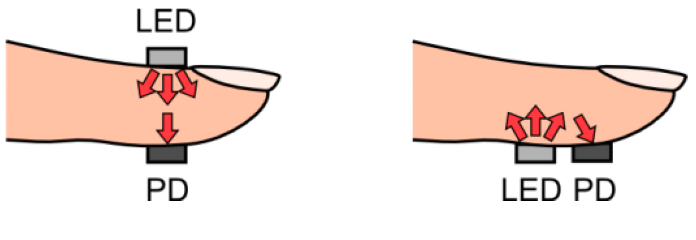
\includegraphics[height=0.2\textheight]{Images/Tamura1.png}

    \citet{takano2007heart}

    Een transmissive PPG kan een relatief goed signaal verkrijgen, maar de meetlocatie is beperkt. 
    Om een meting te doen moet de sensor zich op het lichaam bevinden op een plaats waar doorgelaten licht gemakkelijk kan worden gedetecteerd, zoals de vingertop, het neustussenschot, de wang, de tong of de oorlel. 
    Het plaatsen van de sensor op het neustussenschot, de wang of de tong is alleen effectief onder anesthesie. 
    De vingertop en de oorlel zijn de voorkeursposities; deze plaatsen hebben echter een beperkte bloedperfusie. 
    Bovendien zijn de vingertop en de oorlel gevoeliger voor extreme omstandigheden, zoals lage omgevingstemperaturen.

    Een Reflective PPG elimineert de problemen die verband houden met de plaatsing van de sensor en er kunnen verschillende meetlocaties worden gebruikt (zoals besproken in de volgende sectie). 
    Reflective PPG wordt echter beïnvloed door bewegingsartefacten en druk storingen. 

    \subsection{Hartslag}
    Op eenzelfde manier kan de hartslag worden gemeten. 
    Volgens [Heart rate monitoring system using finger tip through Arduino and Processing Software] zetten de haarvaten in de huid van een vinger op als gevolg van een stijging in de bloeddruk tijdens een hartslag. 
    Deze verandering in formaat kan worden gemeten d.m.v. PPG.

    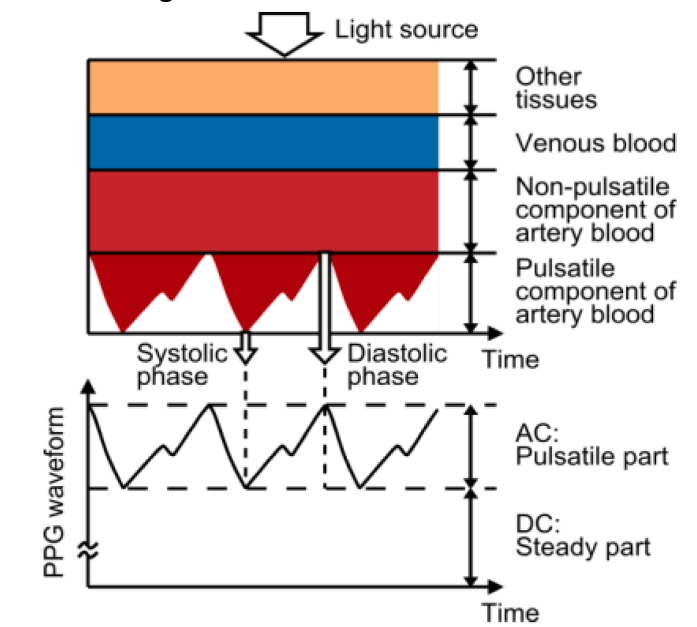
\includegraphics[height=0.5\textheight]{Images/Tamura2.png}

    
    Hartslag is een minstens zo belangrijke metriek als zuurstofsaturatie. Het is algemeen bekend dat zowel een te lage, te hoge als een onregelmatige hartslag kunnen negatieve gevolgen hebben voor de gezondheid. 
    Ook kan er op deze manier vastgesteld worden of de patiënt überhaupt een hartslag heeft.
    Daarnaast is het vaststellen van een hartaanval ook mogelijk door het meten van de onderlinge tussenposes. 

    Te hoge hartslag kan een indicatie zijn van onder andere bloedverlies, koorts, infectie, gebrek. 
    Deze oorzaken zijn veelvoorkomend tijdens rampsituaties aangezien lichamelijke letsel een veel voorkomend gevolg is van een rampsituatie. 
    De gevolgen van een te hoge hartslag zijn kortademigheid, duizeligheid, flauwvallen, zwakte en moeheid.
    [Symptoom Snelle regelmatige hartslag (tachycardie) - Symptomenchecker]

    Te lage hartslag is ook een belangrijke metriek. 
    Dit kan onder andere dienen als indicatie van onderkoeling, bloedingen en een verhoogde hersendruk, naast andere oorzaken. 
    Een te lage hartslag kan leiden tot duizeligheid, kortademigheid, vermoeidheid, hartkloppingen, flauwvallen, en geheugenstoornissen. 
    [Bradycardie (te lage hartslag) - hoe herken je het?]

    misschien nog iets over pleth waves als we dit verder gebruiken.



    \section{Uitvoering}\label{sec:uitvoering}
    \todo{TODO, ik heb dit overgenomen uit het onderzoeksvoorstel, akkoord zo?}
    \subsection{Theorie bloed zuurstofsaturatie en hartslag}
    Voor de lichte verwerking van de data, die deze module zal doen, is een klein beetje context nodig.
    Het gaat hier dan met name om de medische betekenis van de twee waarden die hier worden onderzocht.
    Er zal geen complete diagnose gesteld worden, maar het is niet onbelangrijk om overzicht te houden in de verworven data.
    De patiënten zou bijvoorbeeld kunnen worden gesorteerd op de afwijking van hun data ten opzichte van de verwachte data voor een gezond gemiddeld mens.

    Op deze manier kunnen in ieder geval de op het eerste gezicht meer kritieke gevallen het eerst aan de medici voorgelegd worden.

    Hiervoor zal een stuk onderzoek gedaan moeten worden naar de gezonde bereiken voor de hartslag en zuurstofsaturatie en de gevolgen van het afwijken van die waarden.
    Wellicht resulteert een sterke afwijking in zuurstofsaturatie sneller tot ernstige hulpbehoevendheid dan een sterke afwijking in de hartslag of vice versa.
    Dit soort informatie is dus essentieel om een goede initiële verwerking van de resultaten mogelijk te kunnen maken, opdat de medici sneller ter plaatse kunnen zijn waar de nood het hoogst is.

    Ook is de theorie achter het doen van de metingen belangrijk voor het vergelijken van sensoren, hierdoor kunnen wij geïnformeerd kijken naar de verschillende specificaties van sensoren, en een beslissing maken over welke het beste past bij onze use case.

    \subsection{Van bestaand Proces naar autonome metingen}
    We gaan kijken naar hoe deze metingen worden gedaan in de gezondheidszorg, en wat de procedure is en welk materiaal hiervoor wordt gebruikt.
    Op basis van de kennis die wij opdoen tijdens dit literatuuronderzoek gaan wij dit proberen toe te passen op een module(end effector) die vervolgens deze metingen zo autonoom mogelijk gaat uitvoeren.

    \subsection{Wat maakt een sensor geschikt?}
    Tijdens het literatuuronderzoek over het meten van de Hartslag en Zuurstofsaturatie komen we meer te weten over hoe deze metingen precies worden gedaan, en dus ook welke specificaties van belang zijn voor een goede sensor.
    Naast de meting gerelateerde aspecten van de sensor komen wordt er ook gekeken naar de algemene specificaties van een sensor zoals Stroomverbruik, prijs, form factor,beschikbaarheid etc.
    Er moet gekeken worden bij verschillende chipmakers, distributeurs en bestaande oplossingen om te zien welke sensoren op de markt zijn.


    \section{Resultaten}\label{sec:resultaten}
    \todo{TODO, resultaten verzamelen}

    
    \section{Conclusie en Discussie}\label{sec:conclusie-en-discussie}
    \todo{TODO, wat kan er worden geconcludeerd uit dit onderzoek}


    \section{Evaluatie}\label{sec:evaluatie2}
    \todo{TODO, wat voor problemen kwam je tegen tijdens het onderzoek}

    \section{Aanbevelingen}\label{sec:aanbevelingen2}
    \todo{TODO, wat zijn de aanbevelingen uit dit onderzoek}


    \section{Suggesties voor verder onderzoek}\label{sec:suggesties-voor-verder-onderzoek2}
    \todo{TODO, wat zijn verdere onderzoekssuggesties}


    \section{Literatuur}\label{sec:literatuur2}
    \todo{TODO}
    In dit hoofdstuk beschrijven we de onderzochte literatuur.
    Hierbij geven wij aan wat de relevantie is tot ons eigen onderzoek.



    

    \bibliography{Include/Main}

\end{document}
